As already mentioned, due to fundamental quantum principles exploited by this
protocol, it can be assured once a raw copy of the key bits has been obtained, that no
data has been tapped.
An unavoidable problem with classical communication is the man-in-the-middle attack,
commonly known up to now as eavesdropping. It is an attack on a communication channel where a
third party, Eve, makes independent connections with other parties and relays messages between
them, giving the impression that they are communicating directly to each other. Let Alice
and Bob (as usual) be two parties who wish to communicate over a channel and let the eavesdropper
Eve (as usual, again) be the third party who wishes to intercept the conversation. 
Initially, Alice requests Bob's public key. Bob sends the key, but Eve is able to intercept it. 
Eve then passes her own public key onto Alice, claiming to be Bob. 
Alice encrypts the message with Eve's key and passes the encrypted message onto Eve (unknowingly). 
Eve then decrypts the message and encrypts it with Bob's public key. 
When Bob receives the message, he believes it is coming directly from Alice.

For the sake of understanding how Alice and Bob are safe from Eve, let us play devil's advocate 
by assuming her position.
By pretending to be Eve, we will try to obtain the information intended for
Bob, but secretly (without being detected). 
Thus, according to what has been mentioned so far, if we intercept a polarized photon 
(being sent from Alice to Bob) and make a polarization measurement upon it, Bob will
simply receive a useless piece of data (post-measurement qubits are said to be destroyed).
With that in mind, a smarter post-measurement move would be to resend a photon 
to Bob (so its superposition does not collapse) with the polarization basis 
just used to measure the previous one, so that if it ``survives" {\it sifting} and makes it 
to the final, accepted key (communicated on the public channel), we will know that the qubit 
we spied on was part of the key.
What Bob can do, faced with such a problem, is to sacrifice a randomly chosen subset of
qubits of the ``sifted key" (the one they agreed on, after the first sifting) and
send the remaining subset to Alice through the public channel. Once Alice receives the
remaining subset, she will be able to determine whether or not the initial key was
eavesdropped, by the second process; ``error correction".
How does it work?
``Error" correction simply utilizes the fact that there are cases when Eve
happens to choose a different polarization orientation (resend basis) than the one chosen
by Alice (encoding basis). Such cases are ``Datum" $2$, $4$ and $5$ of Fig. \ref{fig5}.
\begin{figure}[!h]
\centerline{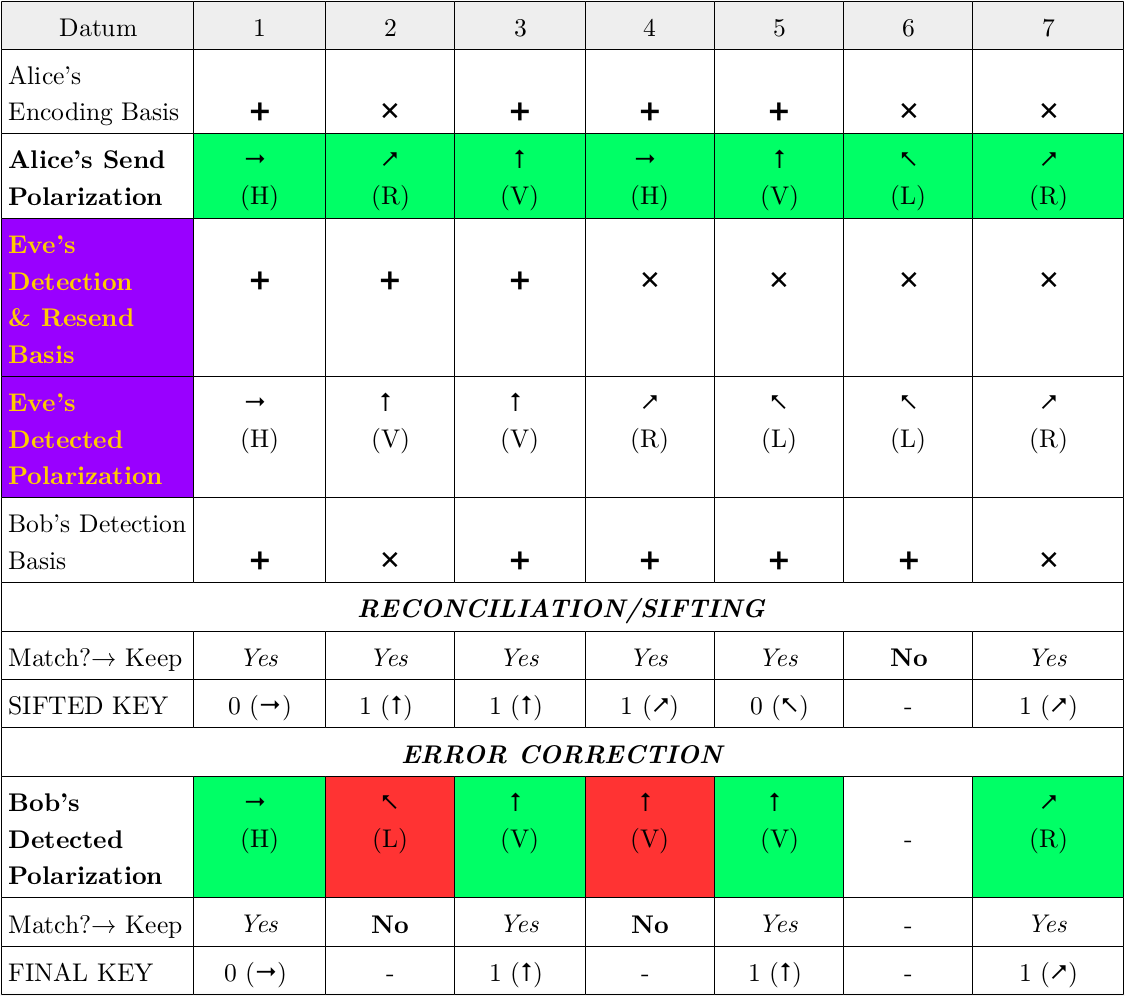
\includegraphics[width=1.4\textwidth,height=1.5\textheight,keepaspectratio]{5.png}}
\caption{An example of realistic QKD (note: for error correction the whole sifted key is used - instead of some subset of it)}
\label{fig5}
\end{figure}
Remember, that prior to {\it error correction}, the qubits that Alice and Bob hold are a randomly selected 
subset of the {\it sifted key}.
In the Fig. \ref{fig5} example and in general, the fact that the result measured by Eve is random is combined
with the fact that in half of the cases, Alice finds a wrong polarization in Bob's qubits
despite their corresponding bases being identical!
The accepted qubits form the final key.
See, for instance, the cases of ``Datum" $2$ and $4$.
If the number of errors surpass a predefined error-rate threshold, Alice warns Bob about Eve and that key is discarded.

To summarize, we must keep in mind the specific property that is at the core of the BB84
protocol, namely the impossibility of finding (by using a measurement basis), 
the polarization of a single photon if the basis that was used to polarize it (polarization basis), 
to begin with, is not know, which, combined with the no-cloning theorem, render this protocol provably secure.
